\documentclass{article}
\setlength{\parskip}{5pt} % esp. entre parrafos
\setlength{\parindent}{0pt} % esp. al inicio de un parrafo
\usepackage{listings} % listings
\usepackage{color} %colores
\usepackage{amsmath} % mates
\usepackage[sort&compress,numbers]{natbib} % referencias
\usepackage{url} % que las URLs se vean lindos
\usepackage[top=15mm,left=20mm,right=20mm,bottom=25mm]{geometry} % margenes
\usepackage{hyperref} % ligas de URLs
\usepackage{graphicx} % poner figuras
\usepackage[spanish]{babel} % otros idiomas

\author{Claudia Lizeth Hern\'andez Ram\'irez} % author
\title{Homework 6 - Multiagente} % titulo
\date{\today}

\definecolor{mypurple}{rgb}{0.305, 0.066, 0.592}
\definecolor{mygray}{rgb}{0.976, 0.980, 0.980}
\definecolor{myorange}{rgb}{0.933, 0.305, 0.090}
\lstset{ 
  backgroundcolor=\color{mygray},
  commentstyle=\color{myorange},
  keywordstyle=\color{mypurple}, 
  numberstyle=\tiny\color{myorange}
  stringstyle=\color{mypurple}, 
  breaklines=true,
}


\begin{document} % inicia contenido

\maketitle % cabecera

% RESUMEEEEEEEEEEEEEEEN
\begin{abstract} % resumen
  \centering
Existe una disminuci\'on en la cantidad de personas contagiadas conforme aumenta la probabilidad de que haya personas vacunadas.
  
\end{abstract}


% INTRODUCCIOOOOOOOOOOOON
\section{Introducci\'{o}n}\label{intro} % seccion y etiqueta
Vacuna con probabilidad \texttt{pv} a los agentes al momento de crearlos de tal forma que están desde el inicio en el estado R y ya no podrán contagiarse ni propagar la infección. Estudia el efecto estadístico del valor \texttt{pv} de  en (de cero a uno en pasos de 0.1) el porcentaje máximo de infectados durante la simulación y el momento (iteración) en el cual se alcanza ese máximo.



% DESARROLLOOOOOOOOOOOO
\section{Desarrollo}\label{desarrollo} % Desarrollo de la tarea

Comenc\'e trabajando con el c\'odigo proporcionado en clase \cite{Cbase}. Como parte de la tarea, deb\'iamos incluir una variaci\'on en la probabilidad de vacunaci\'on inicial, todo en un rango de \texttt{0} a \texttt{1} en pasos de \texttt{0.1}.

\begin{lstlisting}[language=R, caption= Segmento de c\'odigo para variar probabilidad de vacuna inicial.]

l <- 1.5 #Ancho de mi cuadrito
n <- 25 #individuos de mi poblacion
pi <- 0.05 #Probabilidad inicial de infeccion
pr <- 0.02 #Probabilidad de recuperacion
v <- l / 30 #Velocidad con la que se mueven mis individuos
pv = seq(0, 0.9, 0.1) #probabilidad de vacunados
rep = (1:15)
datos = data.frame()

for (vac in pv) { #incremento en la probabilidad de vacunados
  for (arep in rep) { # replicas
\end{lstlisting}


Posteriormente se gener\'o un \texttt{data.frame} en el cu\'al se guardar\'ia la información que se analizar\'a estad\'isticamente.
\begin{lstlisting}[language=R, caption= Segmento de c\'odigo para generar data frame.]

porcentaje<-(maxinf/n)*100
    datos <- rbind(datos,c(vac, maxinf, porcentaje, iteracion)) #data frame 
    names(datos)<-c("probabilidad", "maxinf", "porcinf","tiempo")
\end{lstlisting}


Como es debido, se realizaron pruebas de normalidad para mis datos.



\bigskip
\bigskip


\begin{lstlisting}[language=R, caption= Segmento de c\'odigo para prueba de normalidad Shapiro-Wilk.]
#Estadistica prueba de normalidad - 
      #con p menor a 0.05 se rechaza hipotesis nula H0
      #H0: los datos proceden de una distribucion normal
      #H1: los datos no proceden de una distribucion normal
tapply(datos$maxinf, datos$probabilidad, shapiro.test)
\end{lstlisting}

De esta prueba se obtuvieron los datos expresados en el cuadro \ref{cuadro 1} (Considerando que en la literatura podemos encontrar que diversos autores establecen que en pruebas de normalidad para aceptar la hip\'otesis nula el valor de \texttt{P} debe ser mayor al 0.05, es decir mayor al 5\%).

\begin{table}[ht]
    \centering
    \caption{Resultados obtenidos de prueba de normalidad de Shapiro.} 
    \begin{tabular}{|c|c|c|c|}
    \hline
    Prob. de vacuna & W value & P value & ¿Se acepta H0?  \\
    \hline
    0 & 0.828 & 0.00874 & no \\
    \hline 
     0.1 & 0.835 & 0.01104 & no  \\
    \hline 
    0.2 & 0.849 & 0.01681 & no \\
    \hline 
    0.3 & 0.883 & 0.05264 & si \\
    \hline 
    0.4 & 0.896 & 0.08318 & si \\
    \hline 
    0.5 & 0.743 & 0.00076 & no \\
    \hline 
    0.6 & 0.883 & 0.05274 & si \\
    \hline 
    0.7 & 0.905 & 0.1135 & si \\
    \hline 
    0.8 & 0.866 & 0.02973 & no \\
    \hline 
    0.9 & 0.916 & 0.1728 & si \\
    \hline 
\end{tabular}
    \label{cuadro 1}
\end{table}

Con la informaci\'on obtenida en las pruebas de normalidad, podemos seguir con la prueba estad\'istica. En esta ocasi\'on recurriremos a la prueba de \texttt{Kruskal-Wallis} \cite{Kruskal}.

\begin{lstlisting}[language=R, caption= Segmento de c\'odigo para prueba de Kruskal-Wallis]
#PRUEBA ESTADISTICA
datos%>%
  group_by(probabilidad) %>%
  summarise(
      cantidad_de_participantes = n(),
      promedio = mean(maxinf, na.rm = TRUE),
      desviacion_estandar = sd(maxinf, na.rm = TRUE),
      varianza = sd(maxinf, na.rm = TRUE)^2,
      mediana = median(maxinf, na.rm = TRUE),
      rango_intercuartil =  IQR(maxinf, na.rm = TRUE)
  )

kruskal.test(maxinf ~ probabilidad, data = datos)
pairwise.wilcox.test(datos$maxinf, datos$probabilidad)
\end{lstlisting}
De donde se obtuvieron los resultados expresados en el cuadro \ref{cuadro 2}.

\begin{table}[ht]
    \centering
    \caption{Resultados obtenidos de prueba Kruskal-Wallis.} 
    \begin{tabular}{|c|c|c|}
    \hline
    Chi cuadrada & DF & P  \\
    \hline
    4.2541 & 9 & 0.8939 \\
    \hline
\end{tabular}
    \label{cuadro 2}
\end{table}

\begin{table}[ht]
    \centering
    \caption{Diferencias entre grupos. Kruskal-Wallis.} 
    \begin{tabular}{|c|c|c|c|c|c|c|c|c|c|}
    \hline
    "" & 0 & 0.1 & 0.2 & 0.3 & 0.4 & 0.5 & 0.6 & 0.7 & 0.8 \\
    \hline
    0.1 & 1 & "" & "" & "" & "" & "" & "" & "" & "" \\
    \hline
    0.2 & 1 & 1 & "" & "" & "" & "" & "" & "" & "" \\
    \hline
    0.3 & 1 & 1 & 1 & "" & "" & "" & "" & "" & "" \\
    \hline
    0.4 & 1 & 1 & 1 & 1 & "" & "" & "" & "" & "" \\
    \hline
    0.5 & 1 & 1 & 1 & 1 & 1 & "" & "" & "" & "" \\
    \hline
    0.6 & 1 & 1 & 1 & 1 & 1 & 1 & "" & "" & "" \\
    \hline
    0.7 & 1 & 1 & 1 & 1 & 1 & 1 & 1 & "" & "" \\
    \hline
    0.8 & 1 & 1 & 1 & 1 & 1 & 1 & 1 & 1 & "" \\
    \hline
    0.9 & 1 & 1 & 1 & 1 & 1 & 1 & 1 & 1 & 1 \\
    \hline
\end{tabular}
    \label{cuadro 3}
\end{table}


\begin{table}[ht]
    \centering
    \caption{Informaci\'on individual de los datos.} 
    \begin{tabular}{|c|c|c|c|c|c|c|}
    \hline
    Probabilidad & Qty. Participantes & promedio & Desv. Std. & Varianza & Mediana & Rango Intercuartil  \\
    \hline
    0 & 15 & 4.4 & 5.03 & 25.3 & 2 & \\
    \hline
    0.1 & 15 & 2.67 & 2.97 & 8.81 & 1 & \\
    \hline
    0.2 & 15 & 3.47 & 3.78 & 14.3 & 3 & \\
    \hline
    0.3 & 15 & 3.4 & 3.31 & 11.0 & 3 & \\
    \hline
    0.4 & 15 & 2.73 & 2.31 & 5.35 & 3 & \\
    \hline
    0.5 & 15 & 2.13 & 2.80 & 7.84 & 1 & \\
    \hline
    0.6 & 15 & 1.67 & 1.35 & 1.81 & 2 & \\
    \hline
    0.7 & 15 & 2.4 & 1.84 & 3.4 & 2 & \\
    \hline
    0.8 & 15 & 2.0 & 1.93 & 3.71 & 2 & \\
    \hline
    0.9 & 15 & 1.87 & 1.30 & .70 & 2 & \\
    \hline
\end{tabular}
    \label{cuadro 4}
\end{table}

\bigskip

Considerando que 

-Hip\'otesis nula: hay diferencias en el n\'umero de contagiados entre las probabilidades de vacunaci\'on.

-Hip\'otesis alternativa: no hay diferencias en el n\'umero de contagiados entre las variaciones de vacunaci\'on.

-Con un nivel de significancia igual a 0.05

Contamos con evidencia estad\'istica suficiente para aceptar la \texttt{hip\'otesis nula}.



\begin{figure}[ht!] % figura
    \centering
    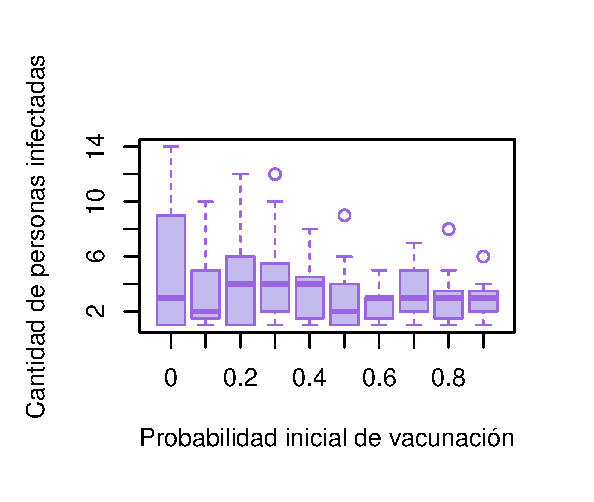
\includegraphics[width=150mm]{infectados.eps} % archivo
    \caption{Variaci\'on de la cantidad de decimales correctas respecto al n\'umero de puntos.}
    \label{Figura 1}
\end{figure}


\begin{figure}[ht!] % figura
    \centering
    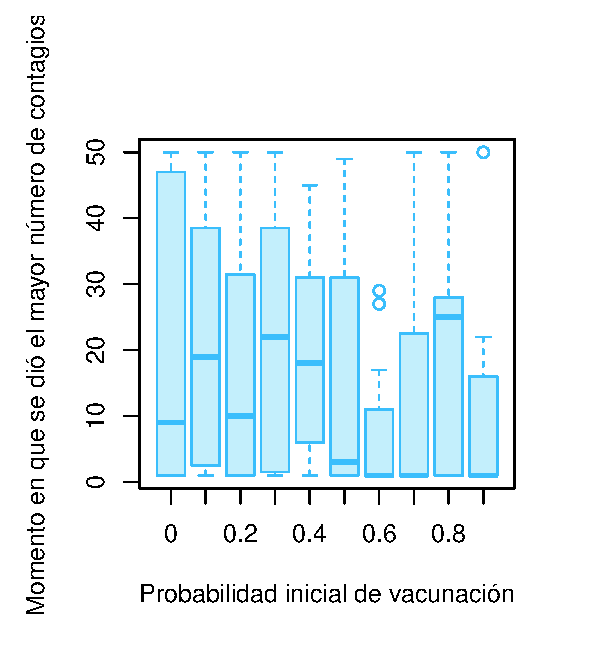
\includegraphics[width=150mm]{tiempo.eps} % archivo
    \caption{Variaci\'on de la cantidad de decimales correctas respecto al n\'umero de puntos.}
    \label{Figura 2}
\end{figure}



%CONCLUSIOOOON
\section{Conclusi\'on}

Es evidente que hay una disminuci\'on en la cantidad de personas contagiadas conforme aumenta la probabilidad de que haya personas vacunadas.
Otra cosa interesante por analizar es el momento en que se presenta el mayor n\'umero de contagios. Se puede apreciar en la figura \ref{Figura 2} hay un amplio rango en el cual se puede presentar el pico de contagios, sin embargo vemos la media en un momento inicial (10) lo cual representar\'ia una saturaci\'on en hospitales y alta demanda de atenci\'on hospitalaria, lo que afecta altamente a los servicios de salud. Observamos que las medias van aumentando conforme aumenta la probabilidad inicial de vacunaci\'on, lo cual tiene l\'ogica, ya que la demanda hospitalaria ser\'a  en un periodo de tiempo mas extendido.


% BIBLIOGRAFIAAAAAAS
\bibliography{referencias}
\bibliographystyle{plainnat}
\end{document}

